\documentclass[a4paper,12pt]{article}
\usepackage{amssymb}
\usepackage{amsfonts}

% Кодировка и язык
\usepackage[utf8]{inputenc}
\usepackage[T2A]{fontenc}
\usepackage[russian]{babel}


% Математические пакеты
\usepackage{amsmath,amsfonts,amssymb}
%Таблицы
\usepackage{array}
\usepackage{booktabs} % Для более красивых горизонтальных линий в таблицах
\usepackage{graphicx}
\usepackage{array}
\usepackage{booktabs}
% Геометрия страницы
\usepackage{geometry}
\geometry{top=2cm, bottom=2cm, left=2.5cm, right=2.5cm}
% Гиперссылки (лучше загружать последним)
\usepackage{hyperref}


% Настройки заголовка
\title{Домашнее задание}
\author{Студент: \textbf{Ростислав Лохов}}
\date{\today}

\begin{document}

% Титульный лист
\begin{titlepage}
    \centering
    \vspace*{1cm}

    \Huge
    \textbf{Домашнее задание}

    \vspace{0.5cm}
    \LARGE
    По курсу: \textbf{Экономика}

    \vspace{1.5cm}

    \textbf{Студент: Ростислав Лохов}

    \vfill

    \Large
    АНО ВО Центральный университет\\
    \vspace{0.3cm}
    \today

\end{titlepage}

% Содержание
\tableofcontents
\newpage

% Основной текст
\section{Сине-Красный уровень}


\subsection{Задача 1}
\begin{enumerate}
    \item $Q^d=Q^s \Leftrightarrow P=60$ т.е при стоимости 60 количество спроса равено количеству предложений
    \item Величина спроса будет равна 30, Величина предложения - 50. Обьем продаж - 30.
\end{enumerate}

\subsection{Задача 2}
А
\begin{enumerate}
    \item Зарубежные поездки - сдвиг cпроса влево 
    \item Рынок турпоездок по России - сдвиг спроса вправо 
    \item Рынок пассажирских перевозок - сдвиг спроса вправо 
    \item Рынок аренды жилья - сдвиг спроса вправо 
\end{enumerate}
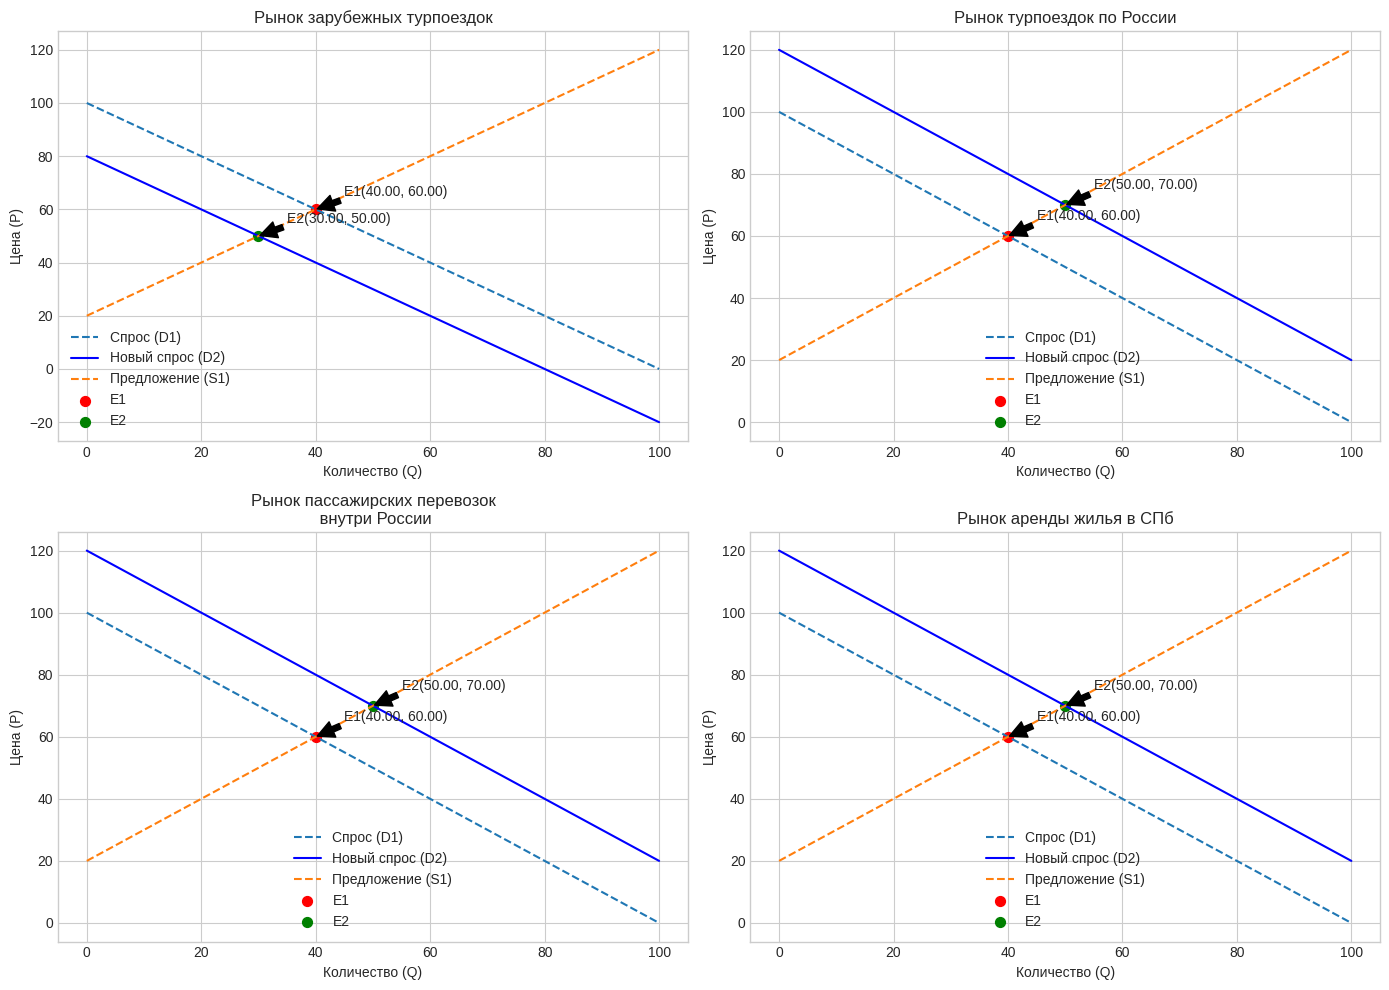
\includegraphics[scale=0.45]{graphs/2.1.png}

Б
\begin{enumerate}
    \item Рынок зарубежных турпоездок. Изменился спрос (т.к зарубежные поездки стали менее привлекательными)
    \item Рынок турпоездок по россии. Изменился спрос (переориентация на внутренний туризм)
    \item Рынок пассажироперевозок. Изменился спрос (увеличился внутренний туризм также)
    \item Рынок аренды жилья. Изменился спрос (также увеличение внутреннего туризма)
\end{enumerate}

В
\begin{enumerate}
    \item Зарубежные турпоездки и турпоездки по России. Когда зарубежные поездки дорожают и становятся менее доступны, тогда потребители переключаются на народный товар - Краснодарский край и Крым. Тогда Субституты. В таком случае Увеличение цены на одно приводит к увеличению цен на другое.
    \item Турпоездки и пассажироперевозки внутри России. Для осуществления турпоездки нужен допустим автобус до местоназначения. Комплемент. Увеличение спроса на одно ведет к увеличению спроса на другое. 
    \item Турпоездки по России и аренда жилья. Если турист выбирает турпоездку в город, то ему нужно жилье для проживания. Следовательно Комплемент. Увеличение спроса на одно ведет к увеличению спроса на другое.
\end{enumerate}

\subsection{Задача 3}

\begin{enumerate}
    \item Повышение
    \item Сокращаются
    \item Вырос
    \item Отток
    \item Продавать
    \item Избыток
    \item Остановить
    \item Ослабления
\end{enumerate}

\subsection{Задача 4}
После прочтения википедии могу кратко резюмировать. У них разрешается есть утром и вечером, притом блюда должны быть праздничные. И существует много социальных активностей с едой. Т.к увеличивается спрос на продукты, то увеличивается и стоимость продажи этих же продуктов

\subsection{Задача 5}
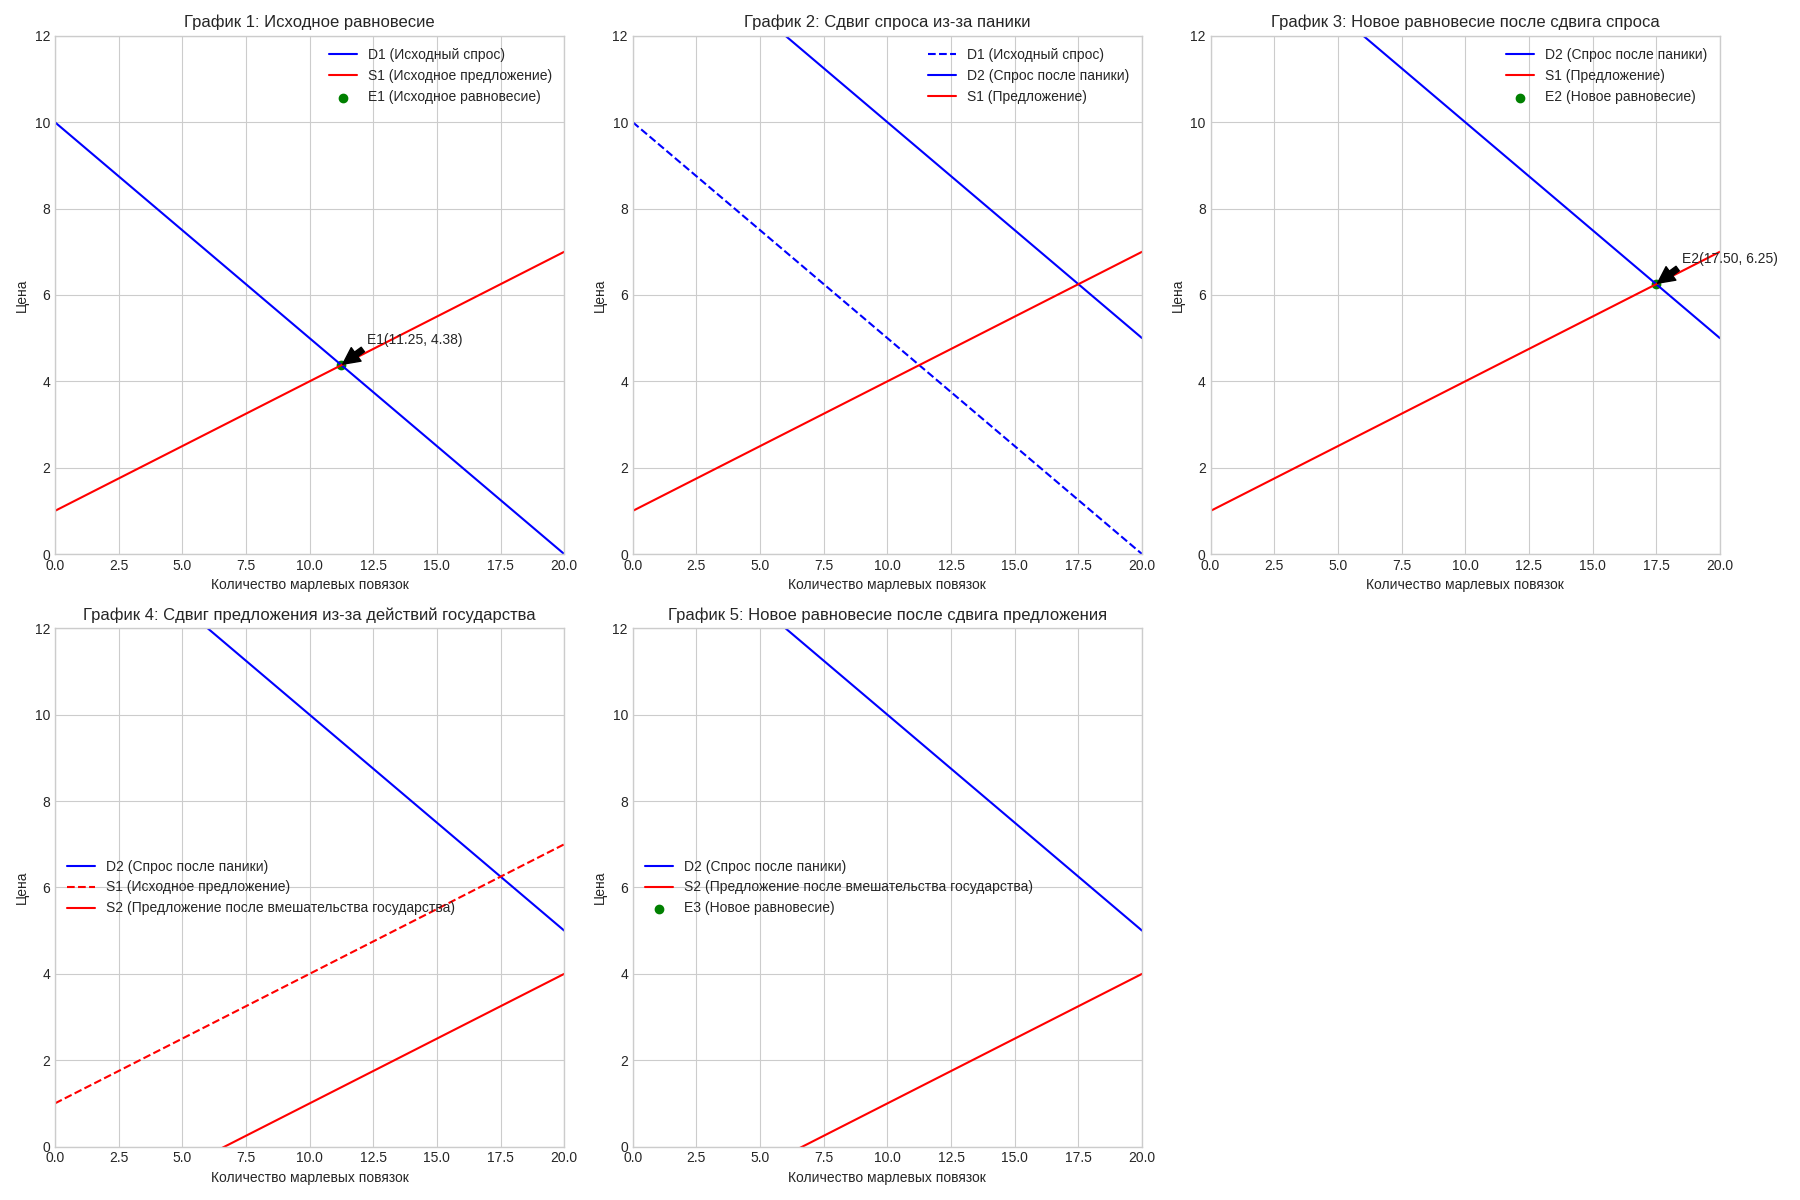
\includegraphics[scale=0.4]{graphs/2.2.png}


\subsection{Задача 6}
\begin{enumerate}
    \item Исландия. Крайне дорогие поставки или производство из за того что страна-остров , ухудшение экономических показателей привело к тому, что стало невыгодно содержать бизнес.
    \item Москва - столица с более дорогим уровнем доходов, большим числом туристов и т.п и т.д. Все производства не надо импортировать. Всё есть, всё рядом. Потому даже в условиях экономического спада рентабельность была положительной.
\end{enumerate}

\subsection{Задача 8}
\begin{enumerate}
    \item $a-220b=40$
    \item $220c-d=40$
    \item $a-219b-219c+d=7$
    \item $220c-d=0$
\end{enumerate}

Решая данную систему линейных уравнений получаем:

\[
a=1140 \land b = 5 \land c = 2 \land d = 400
\]
Таким образом:

\[
Q_d(P) = 1140 - 5P
\]

\[
Q_s(P) = 2P-400
\]

\section{Черный уровень}
\subsection{Задача 1}

Для начала рассмотрим текущую ситуацию.
\begin{enumerate} 
    \item ВВП германии сокращается. Куча проблем, нерабочая стратегия(дешевые энергоносители из рф и доступные рынки).
    \item Усиление конкуренции Китая. Сокращение мировой торговли, Энергетический кризис.
    \item Нехватка населения, квалифицированной рабочей силы, бюрократия, щедрые пособия по безработице, малые инвестиции в технологии.
\end{enumerate}

Теперь рассмотрим модель спроса:

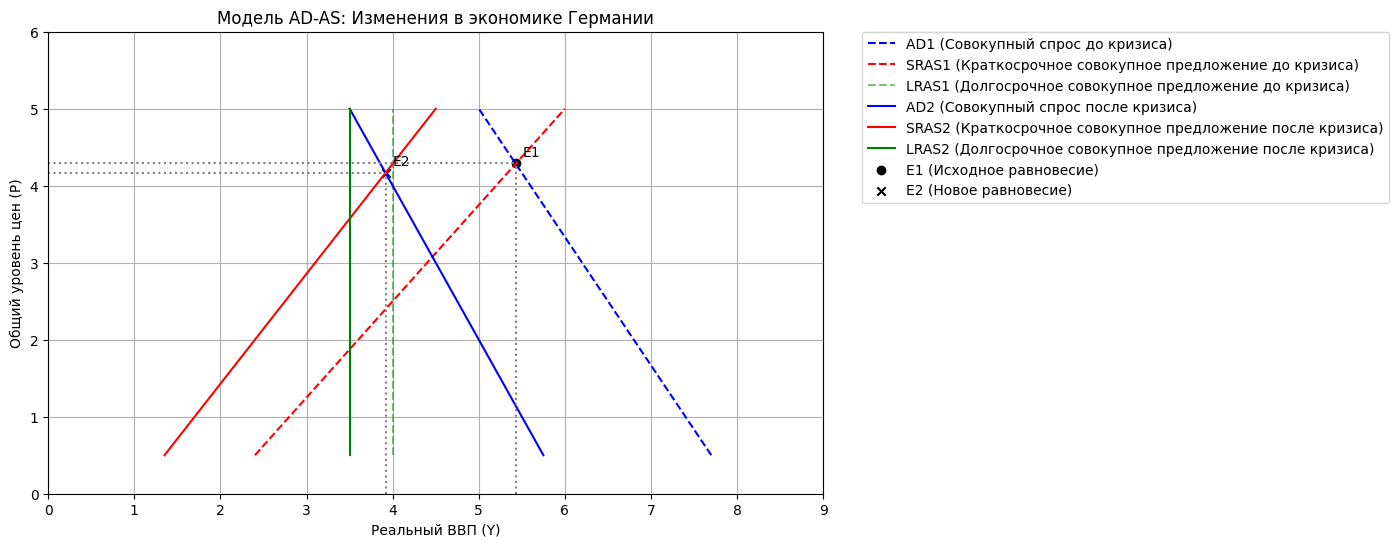
\includegraphics[scale=0.7]{graphs/2.3.png}

Уравнения:

\begin{enumerate}
    \item $x_as1 = 2 + 0.8 * y$
    \item $x_ad1 = 8 - 0.6 * y$
    \item $lras1_{x_i} = 4$
    \item $e1_y = 4.29 $
    \item $e1_x = 5.43$
    \item $x_as2 = 1 + 0.7 * y$
    \item $x_ad2 = 6 - 0.5 * y$
    \item $lras2_x = 3.5 * 100$
    \item $e2_y = 4.17 $
    \item $e2_x = 3.92 $
\end{enumerate}


\subsection{Задача 2}
\begin{verbatim}
    import pandas as pd
    from sklearn.linear_model import LinearRegression
    
    # Данные в виде словаря
    data_dict = {
        'Q, шт.': [736, 821, 682, 817, 708, 849, 735, 789, 813, 823, 828, 696, 807, 772, 784, 802, 772, 696, 761, 675, 646, 784, 731, 848, 715],
        'P ($)': [1.2, 1.2, 1.2, 1.2, 1.2, 1.2, 1.2, 1.2, 1.2, 1.2, 1.2, 1.2, 1.2, 1.2, 1.2, 1.2, 1.2, 1.2, 1.2, 1.2, 1.2, 1.2, 1.2, 1.2, 1.2],
        'курс $': [85.5693, 70.8087, 95.3940, 69.1350, 91.5099, 67.4557, 86.5669, 80.0065, 77.2545, 74.4838, 67.7163, 90.8326, 74.0743, 79.7249, 76.2018, 73.9957, 82.1286, 97.1002, 85.1739, 96.8484, 98.5313, 78.9472, 87.7202, 69.4496, 94.1684]
    }
    
    # Создаем DataFrame из словаря
    df = pd.DataFrame(data_dict)
    
    # Рассчитываем рублевую цену продукта
    df['Р (руб.)'] = df['P ($)'] * df['курс $']
    
    # Выводим таблицу
    print(df)
    
    # Выделяем признаки (X) и целевую переменную (y)
    X = df[['Р (руб.)']] # Цена в рублях - признак
    y = df['Q, шт.']      # Величина спроса - целевая переменная
    
    # Создаем и обучаем модель линейной регрессии
    model = LinearRegression()
    model.fit(X, y)
    
    # Получаем коэффициенты модели
    коэффициент_наклона = model.coef_[0]
    свободный_член = model.intercept_
    
    # Выводим уравнение линейной регрессии (функцию спроса)
    print(f"\nПрямая функция спроса (линейная): Q = {коэффициент_наклона:.2f} * P (руб.) + {свободный_член:.2f}")
# OUTPUT:
Q, шт.  P ($)   курс $   Р (руб.)
0      736    1.2  85.5693  102.68316
1      821    1.2  70.8087   84.97044
2      682    1.2  95.3940  114.47280
3      817    1.2  69.1350   82.96200
4      708    1.2  91.5099  109.81188
5      849    1.2  67.4557   80.94684
6      735    1.2  86.5669  103.88028
7      789    1.2  80.0065   96.00780
8      813    1.2  77.2545   92.70540
9      823    1.2  74.4838   89.38056
10     828    1.2  67.7163   81.25956
11     696    1.2  90.8326  108.99912
12     807    1.2  74.0743   88.88916
13     772    1.2  79.7249   95.66988
14     784    1.2  76.2018   91.44216
15     802    1.2  73.9957   88.79484
16     772    1.2  82.1286   98.55432
17     696    1.2  97.1002  116.52024
18     761    1.2  85.1739  102.20868
19     675    1.2  96.8484  116.21808
20     646    1.2  98.5313  118.23756
21     784    1.2  78.9472   94.73664
22     731    1.2  87.7202  105.26424
23     848    1.2  69.4496   83.33952
24     715    1.2  94.1684  113.00208

Прямая функция спроса (линейная): Q = -4.71 * P (руб.) + 1226.97
\end{verbatim}

\subsection{Задача 3}
\begin{enumerate}
    \item $QD = QD_m +QD_f = 150-0.75P$ - Функция рыночного спроса
    \item $QD = QS \Leftrightarrow P = 75 \Leftarrow QD(75)=93.75$ - Равновесная цена и равновесный обьем продаж
    \item $Qd(160)=30 \Leftarrow QS=200$ - Величина рыночного спроса, величина рыночного предложения, также обьем продаж равен 30
\end{enumerate}



\end{document}